\section{The \thisproj{} Framework}
\label{sec:design}


\subsection{The Design}
\label{Principle Model}

\begin{figure}[t]
    \centering
    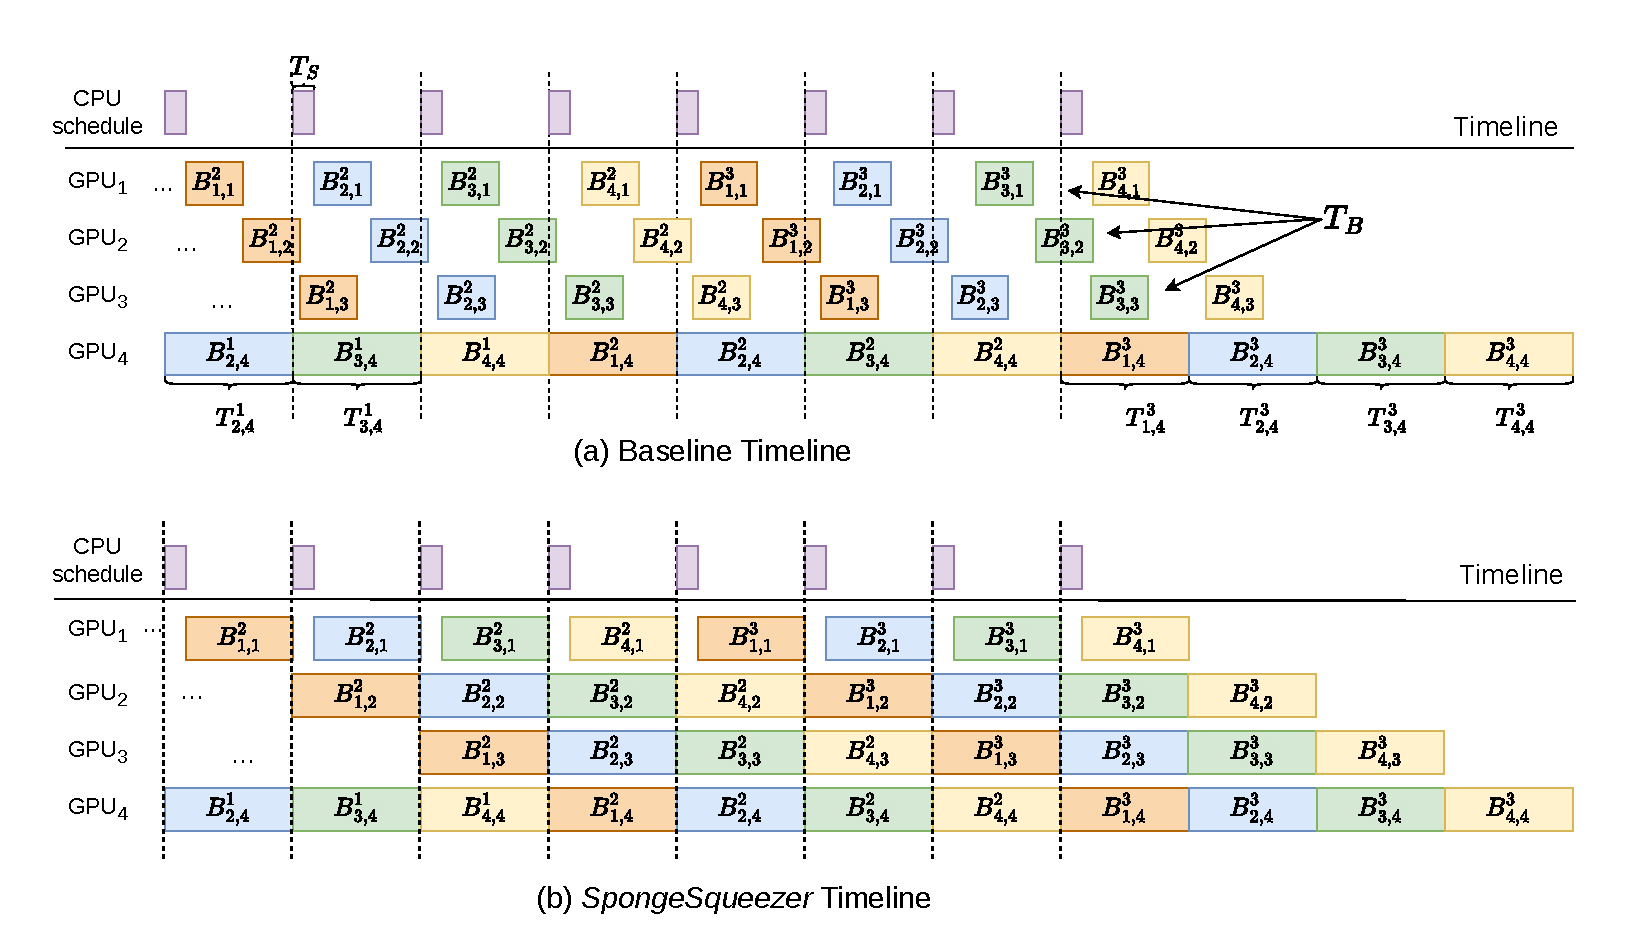
\includegraphics[width=0.9\linewidth]{figures/TACO_Rebuttal/timeline.pdf}
    \caption{(a) The timeline that shows pipeline bubbles in Continuous Batching. (b) The time line that shows \thisproj{} can reduce pipeline bubbles by aligning the stages through frequency adjustment with minimal impact on performance.}
    \label{timeline}
\end{figure}
We ignore the Prefill phase and focus only on the Decode phase, which is the main part of the inference process where pipeline bubbles become unavoidable due to the limited GPU memory capacity.
%To better analyze this phenomenon, 
We extract the part of Decode phase from Figure~\ref{workflow} and show it in Figure~\ref{timeline}(a). 

% We define the process time of an iteration in the batch $i$ on $GPU_j$ (i.e. in stage $j$) as $T_{i,j}$ (see Figure \ref{timeline}(a)).
% For instance, the execution time of any iteration in batch $B_2$ on $GPU_3$, represented by the blue block in the last row, is denoted as $T_{2,3}$.
% The execution time of the scheduler on the CPU side is marked as $T_S$ and depicted as the purple blocks in the first row of the figure. 
% Additionally, we represent the time consumed by pipeline bubbles as $T_B$, which corresponds to the blank areas in the pipeline. 
\bylyz{
We define the processing time of batch $B_{i,j}^{k}$ as $T_{i,j}^{k}$, representing the execution time of batch $i$ on $\text{GPU}_j$ during the $k$-th iteration (see Figure \ref{timeline}(a)).
Let $M$ denote the total number of batches, $N$ the number of GPUs, and $K$ the total number of iterations.
The indices are bounded as follows: $1 \leq i \leq M$, $1 \leq j \leq N$, and $1 \leq k \leq K$.
Additional, the execution time of the scheduler on the CPU side is marked as $T_S$ and depicted as the purple blocks in the first row of the figure. 
We also represent the time consumed by pipeline bubbles as $T_B$, which corresponds to the blank areas in the pipeline. 
}

% An imbalance can be observed in the pipeline stages with the last stage taking significantly longer time than the others. 
% Experimental results indicate that the execution time for all $T_{i,1}$ to $T_{i,n-1}$ is almost the same, while the last stage $T_{i,n}$ is significantly longer, reaching nearly twice that of the earlier stages in the Llama3-8B.
% Consequently, only the last stage of the pipeline remains fully occupied, and the system’s end-to-end latency can be approximated as the cumulative execution time of all batches on $GPU_n$, expressed as:$\sum_{i=1}^{EOS}T_{i,n}$.
% And the bubbles occupy a substantial portion of the total pipeline execution time.
% Specifically, the ratio of the total bubble time to the total execution time is: $$\frac{T_B}{\sum_{i=1}^{EOS}\sum_{j=1}^NT_{i,j}}$$ 

\bylyz{
An imbalance can be observed in the pipeline stages with the last stage taking significantly longer time than the others. 
Experimental results indicate that the execution time for all $T_{i,1}^{k}$ to $T_{i,N-1}^{k}$ is almost the same, while the last stage $T_{i,N}^{k}$ is significantly longer, reaching nearly twice that of the earlier stages in the Llama3-8B.
Consequently, only the last stage of the pipeline remains fully occupied, and the system’s end-to-end inference time can be approximated as the cumulative execution time of all batches on GPU$_N$, expressed as:$\sum_{i=1}^{M}\sum_{k=1}^{EOS}T_{i,N}^{k}$.
And the bubbles occupy a substantial portion of the total pipeline execution time.
Specifically, the ratio of the total bubble time to the total execution time is: $$\frac{\sum{T_B}}{\sum_{i=1}^{M}\sum_{j=1}^{N}\sum_{k=1}^{K}T_{i,j}^{k}}$$ 
}



% T_{i,j} (j=0,...,N-1)
To address this issue, we propose \thisproj{}, a solution that leverages the frequency scaling technology to extend $T_{i,j}^{k}$ by scaling down GPU frequency, thereby lengthening the execution time to fill the bubble time $T_B$. 
%Because individual pipeline bubbles are short-lived and arise from rapid load fluctuations, real-time dynamic adjustments are ineffective at capturing and mitigating them. 
%Instead, \thisproj{} employs a static power adjustment strategy by setting a fixed power limit.
As illustrated in Figure~\ref{timeline}(b), the optimized timeline demonstrates the improvements achieved through this approach. \thisproj{} minimizes pipeline bubbles by aligning the execution time $T_{i,j}^{k}$ across all GPUs to match $T_{i,N}^{k}$. 
Ideally, this adjustment creates a balanced pipeline where every stage has a duration equal to $T_{i,N}^{k}$.
It is important to note that GPU$_1$ must wait for the scheduler to assemble the batch, which adds $T_S$ to the execution time of stage 1.
Consequently, the execution time for the stage on GPU$_1$ is slightly shorter than that of the other GPUs. 
Additionally, as described earlier that the last stage GPU (GPU$_N$) needs to handle other critical tasks, its execution time will directly impact the overall end-to-end inference time. 
To preserve the stability of these critical tasks, \thisproj{} does not adjust the frequency of GPU$_N$.

% There are several techniques to regulate the power thereby adjust the execution time $T_{i,j}^{k}$. 
% These include adjusting the compute core frequency, memory frequency, and the power cap of GPUs. 
% Among them, adjusting the GPU power cap is the simplest approach as it directly limits the GPU's maximum power consumption, which in turn can regulate its performance. 
% The GPU can automatically select the most appropriate power state (p-state) based on the workload to optimize the power/energy efficiency without compromising the performance.

\bylyz{
Modern GPUs provide interfaces to set both maximum and minimum frequency constraints.
In our approach, we configure the maximum and minimum constraints to the exact same value, thereby forcing the GPU to run at a fixed frequency. 
This guarantees that all batches execute under a uniform frequency and mitigates the impact of frequency-induced fluctuations on the stability of stage execution time.
}

% \bygpt{
% On supported GPUs, software interfaces allow the lower and upper bounds of the core frequency to be configured. We set both bounds to the same supported value to request a fixed core frequency. Maintaining this setting across batches on a given GPU helps reduce frequency-induced variation in stage execution time, although the achieved frequency may still be affected by power and thermal limits.
% }

% \bygemini{
% Modern GPUs provide interfaces to set both maximum and minimum frequency constraints. In our approach, we configure the maximum and minimum constraints to the exact same value, thereby forcing the GPU to run at a fixed frequency. This guarantees that all batches execute under a uniform frequency and mitigates the impact of frequency variations on the stability of stage execution times.
% }

% % Figure 8
% \begin{figure}[t]
%     \centering
%     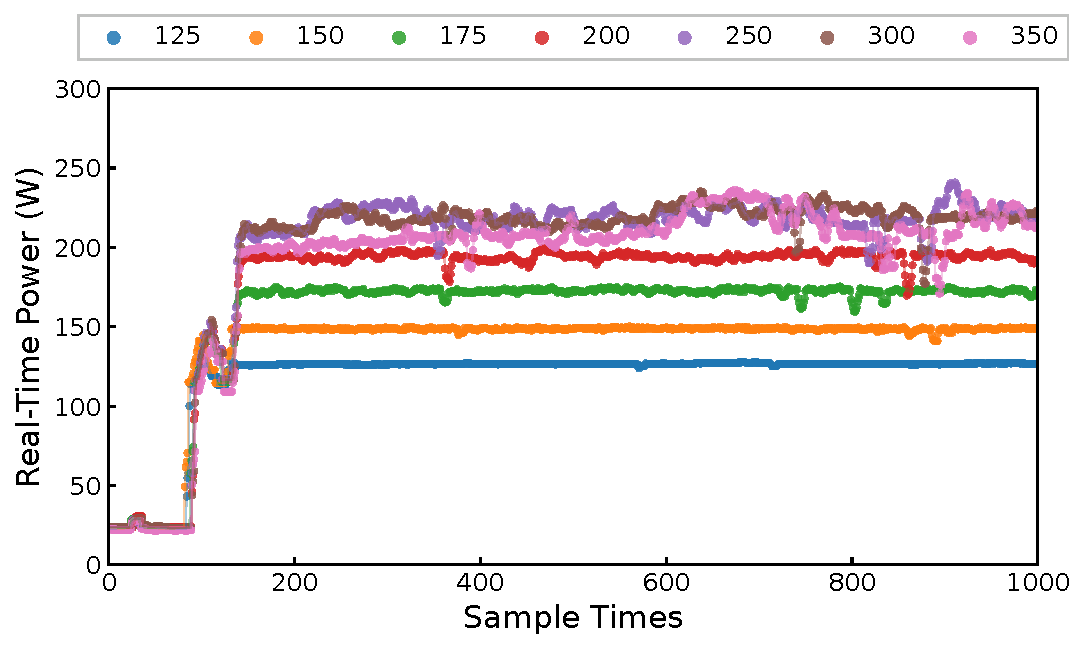
\includegraphics[width=0.8\linewidth]{figures/power_nq_lyz_new_new.pdf}
%     \caption{Real-time power consumption on the Natural Questions dataset using the Llama3-8B model on an RTX 3090 GPU. Different colors represent different GPU power cap settings.}
%     \label{power-runtime}
% \end{figure}

% % Figure 9
% \begin{figure}[t]
%     \centering
%     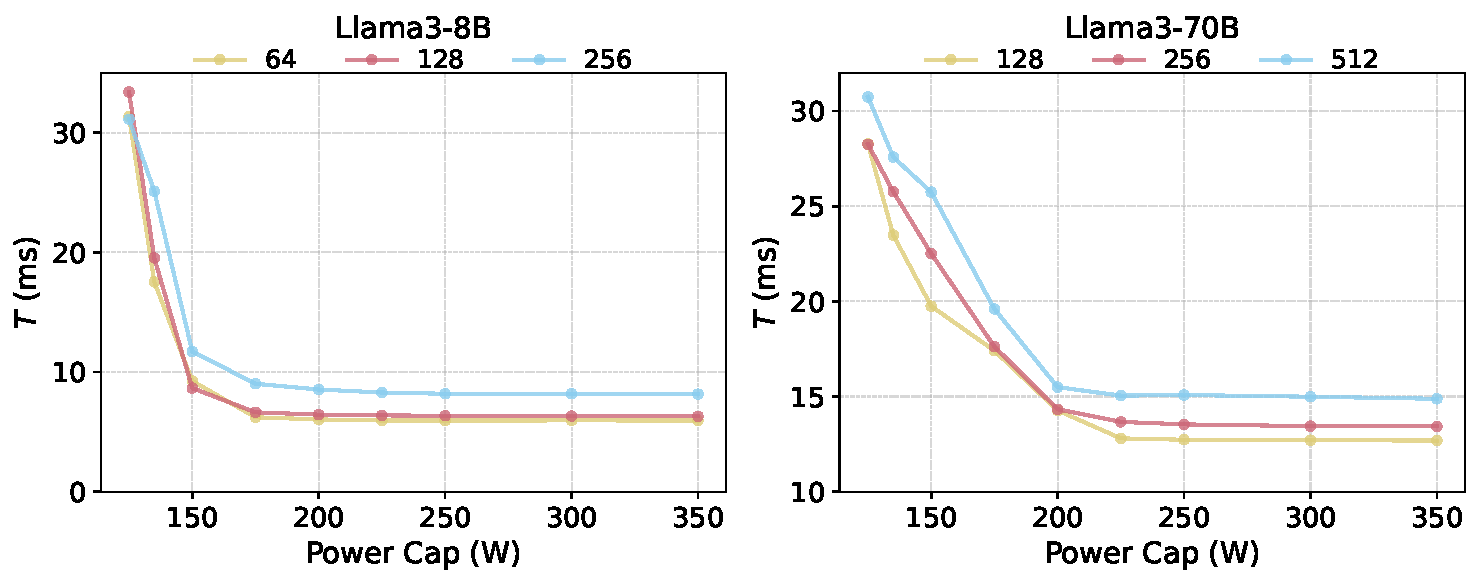
\includegraphics[width=1\linewidth]{figures/execution_time_sampling_new_new.pdf}
%     \caption{Variation of $T$ with different batch size across four Nvidia RTX 3090 GPUs and one NVidia A100 GPU, using Llama3-8B and Llama3-70B on the ShareGPT dataset.}
%     \label{profile_data}
% \end{figure}

% Figure 8 and 9
\begin{figure}[t]
    \centering
    \begin{minipage}[t]{0.48\textwidth}
        \centering
        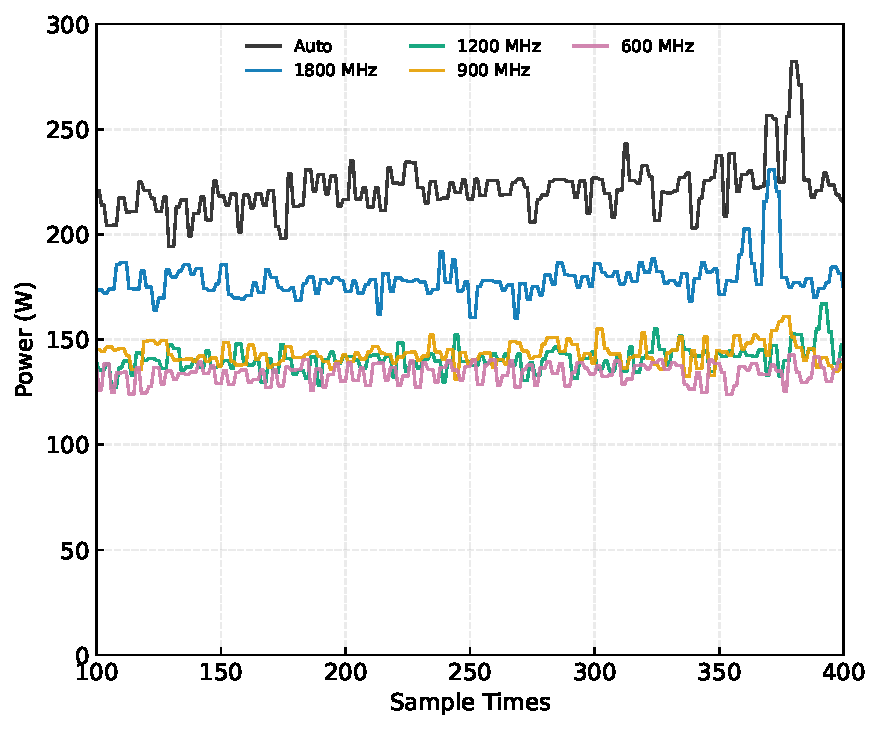
\includegraphics[width=\textwidth]{figures/hcw_final_figures/Fig6_power_sarathi_20261017.pdf}
        \caption{\lyzcheck{Real-time power consumption during inference under various GPU frequency constraints. Different colors represent distinct GPU frequency settings.}}
        \label{power-runtime}
    \end{minipage}
    \hspace{0.02\textwidth}
    \begin{minipage}[t]{0.48\textwidth}
        \centering
        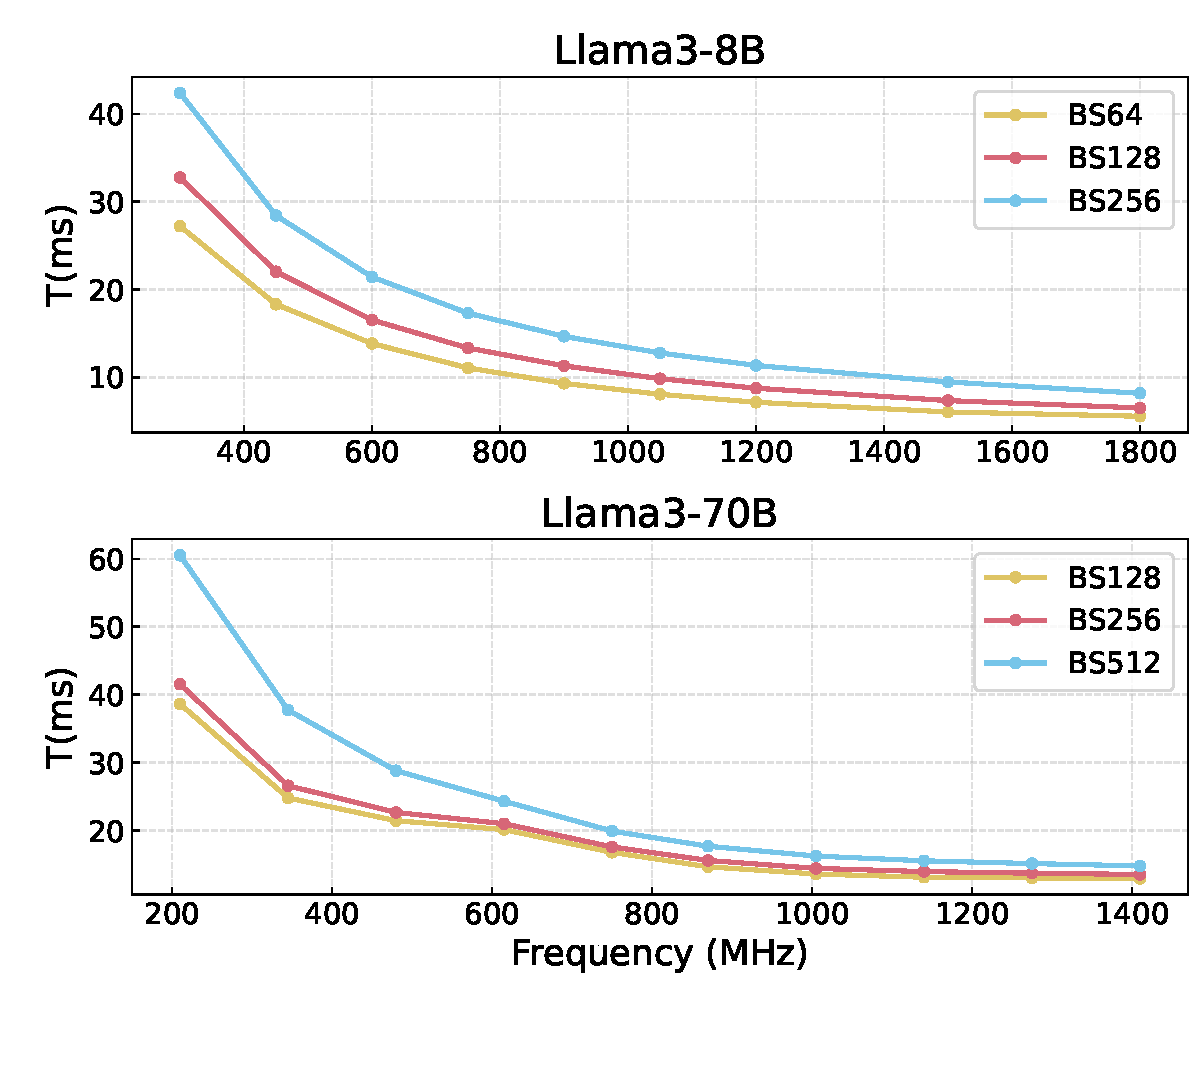
\includegraphics[width=\textwidth]{figures/hcw_final_figures/Fig7_frequency_stage_time_llama_sharegpt_20261018.pdf}
        \caption{\lyzcheck{Variation of $T$ with different batch size across four Nvidia RTX 3090 GPUs and eight Nvidia A100 GPUs, using Llama3-8B and Llama3-70B on the ShareGPT dataset.(The x is $f$, y is $T$. The scatter is the sampled data about $f$ and $T$. Use the line to connect these scatters.)}}
        \label{profile_data}
    \end{minipage}
\end{figure}

% % Figure 8 And 9
% \begin{figure}[t]
%     \centering
%     \begin{minipage}{0.48\textwidth}
%         \centering
%         \raisebox{-\totalheight}{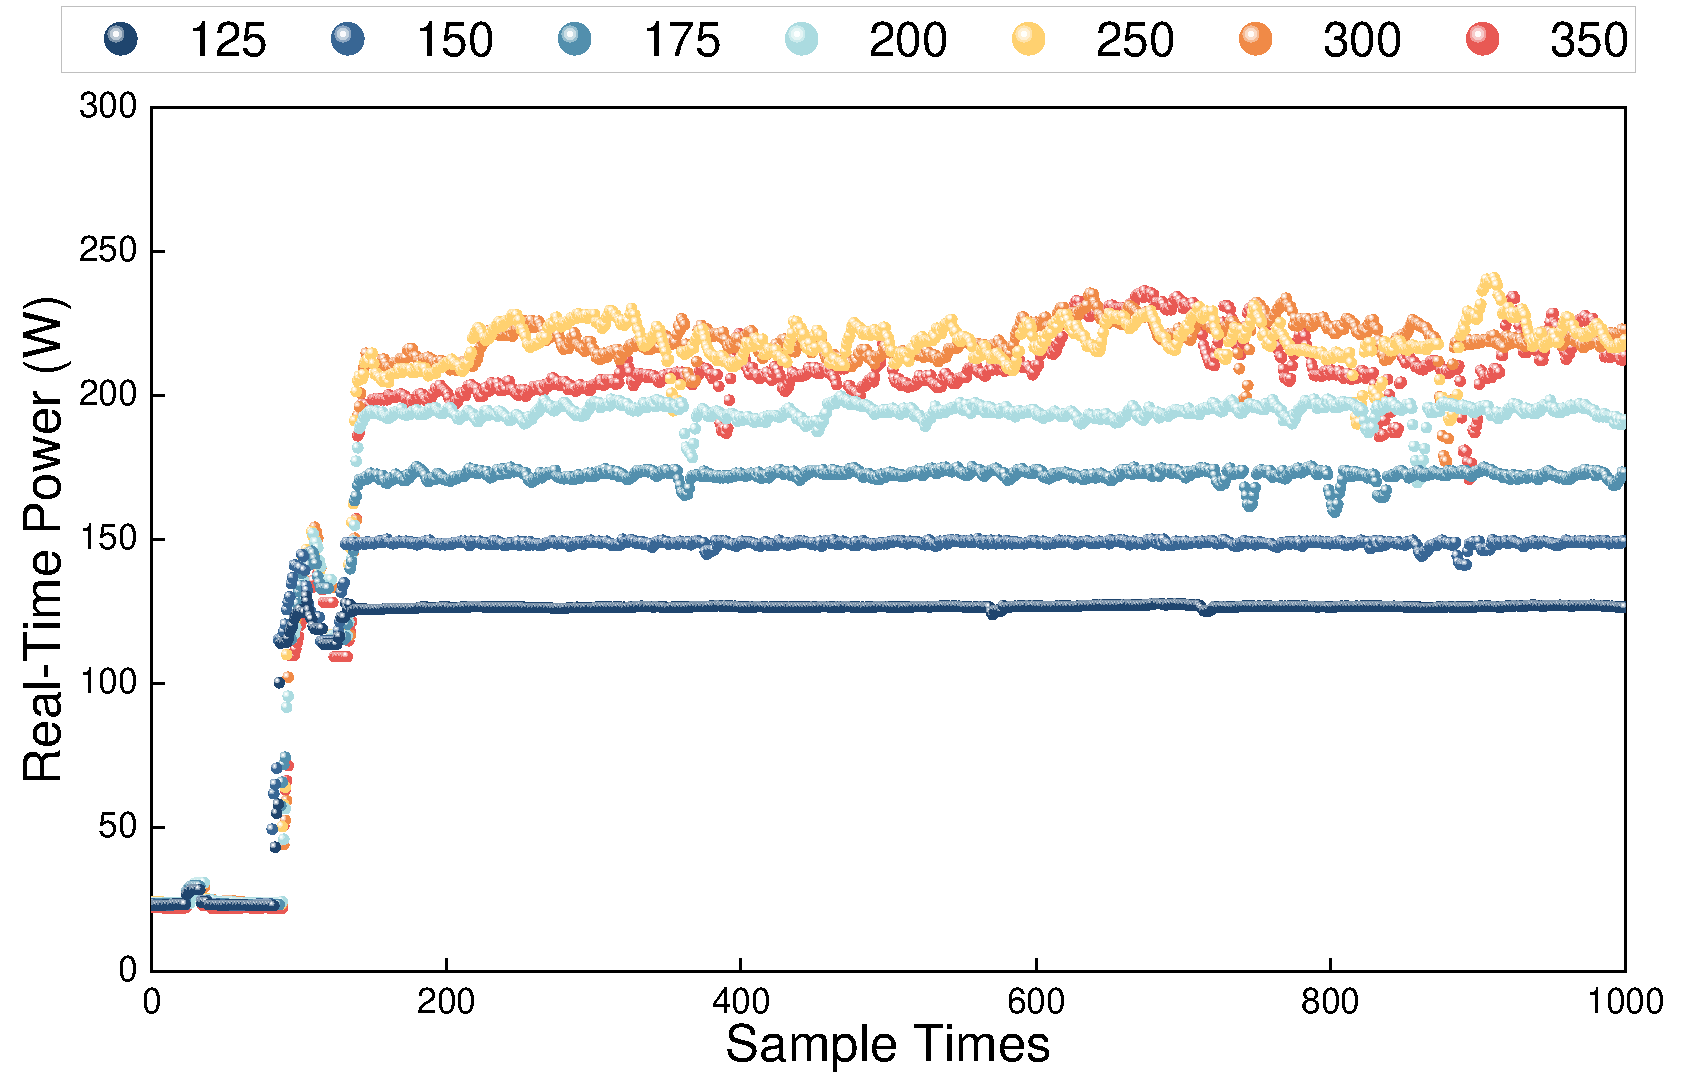
\includegraphics[width=\textwidth]{figures/power_nq_lyz_new.pdf}}
%         \caption{Real-time power consumption on the Natural Questions dataset using the Llama3-8B model on an RTX 3090 GPU. Different colors represent different GPU power cap settings.}
%         \label{power-runtime}
%     \end{minipage}\hfill
%     \begin{minipage}{0.48\textwidth}
%         \centering
%         \raisebox{-\totalheight}{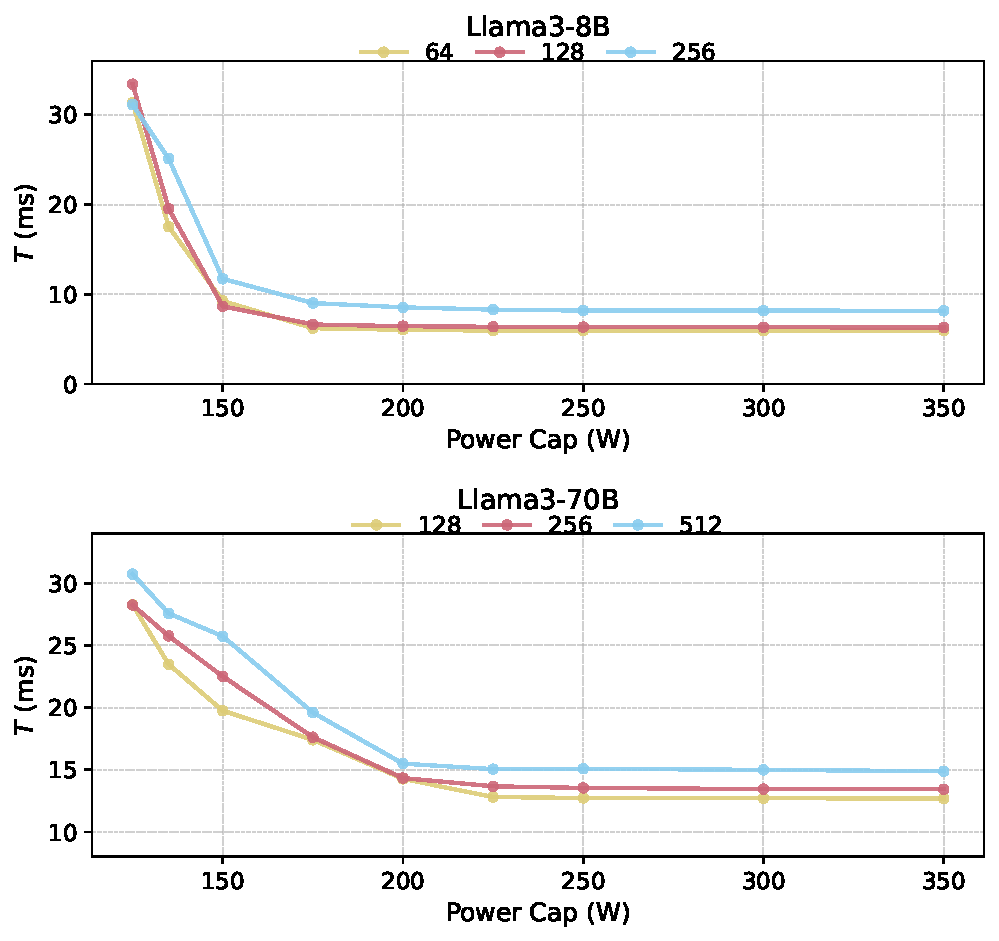
\includegraphics[width=\textwidth]{figures/execution_time_sampling_new_new_new_new.pdf}}
%         \caption{Variation of $T$ with different batch size across four Nvidia RTX 3090 GPUs and one NVidia A100 GPU, using Llama3-8B and Llama3-70B on the ShareGPT dataset.}
%         \label{profile_data}
%     \end{minipage}
% \end{figure}

% \begin{figure}
% 	\centering
% 	\begin{minipage}[t]{\linewidth}
% 		\centering
% 		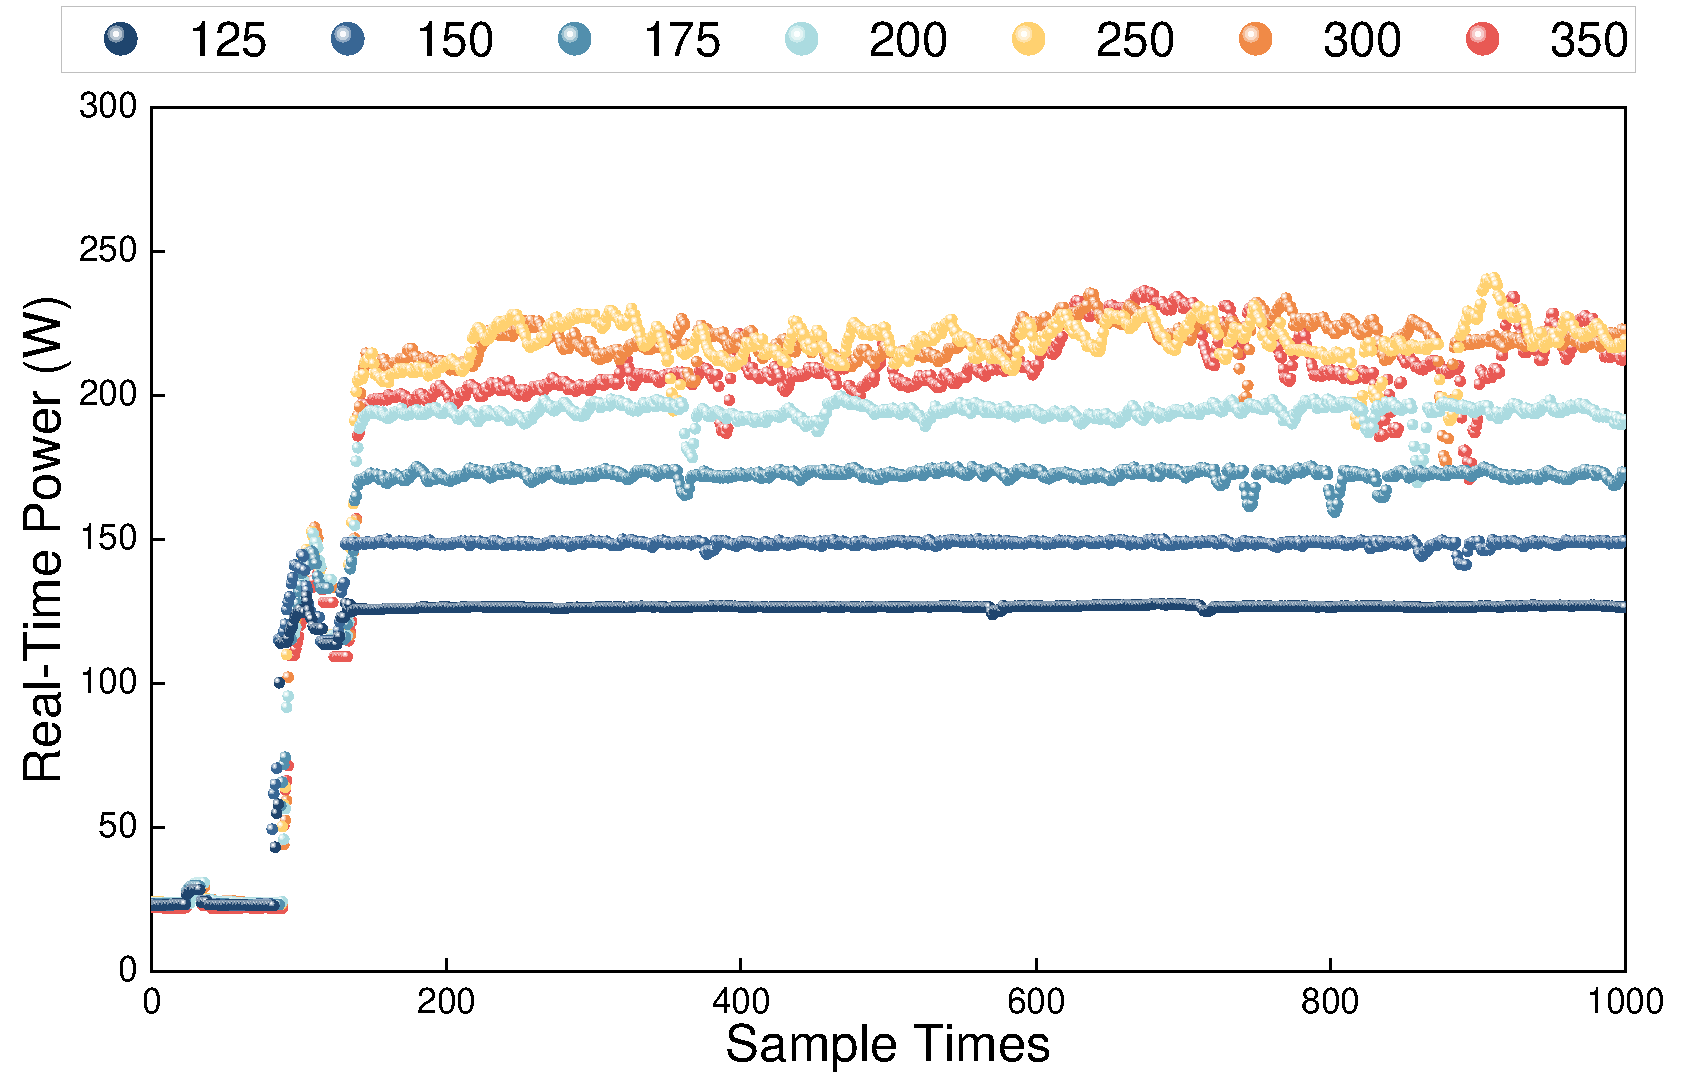
\includegraphics[width=3.3in]{figures/power_nq_lyz_new.pdf}
% 		\caption{Real-time power consumption on the Natural Questions dataset using the Llama3-8B model on an RTX 3090 GPU. Different colors represent different GPU power cap settings.}
% 		\label{power-runtime}
% 	\end{minipage}
% 	\begin{minipage}[t]{\linewidth}
% 		\centering
% 		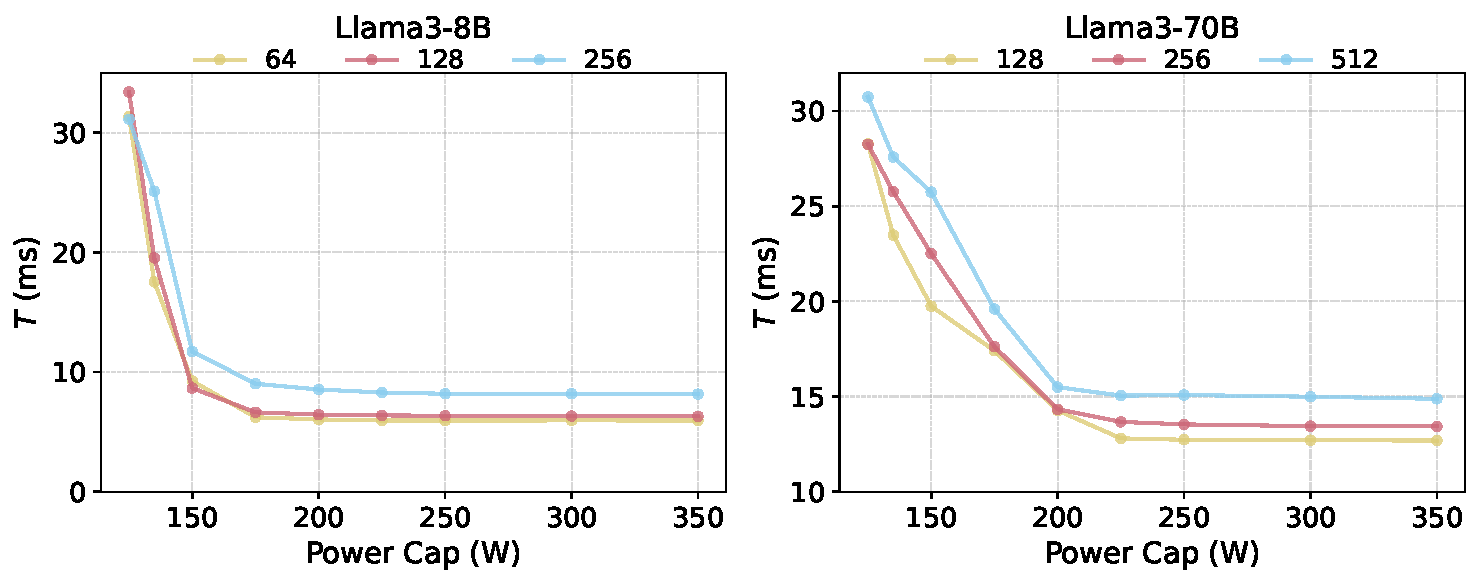
\includegraphics[width=3.3in]{figures/execution_time_sampling_new_new.pdf}
% 		\caption{Variation of $T$ with different batch size across four Nvidia RTX 3090 GPUs and one NVidia A100 GPU, using Llama3-8B and Llama3-70B on the ShareGPT dataset.}
% 		\label{profile_data}
% 	\end{minipage}
%     \label{LLM architecture}
% \end{figure}

% Figure~\ref{power-runtime} illustrates the impact of the power cap on real-time power by sampling actual power consumption during online inference.
% The data is collected during inferences of the Llama3-8B model on RTX 3090 GPUs.
% The results show that the power cap setting operates independently of the DVFS mechanism. 
% By configuring the power cap, the GPU's DVFS mechanism continues to dynamically adjust real-time power based on workload demands.
% At the start of inference, power consumption is relatively low. As the workload increases, power consumption rises significantly while fluctuating slightly within the defined power cap.
% This demonstrates that setting a power cap effectively limits total power consumption without interfering with the normal operation of GPU DVFS, thereby simplifying the design and implementation of \thisproj{}.

\bylyz{
The frequency setting can affect the running power directly.
Figure~\ref{} illustrates the impact of the frequency setting on real-time power by sampling actual power consumption during online inference.
The data is collected during inferences of the Llama3-8B model on RTX 3090 GPUs.
The results show that power consumption follows the same trend as frequency, where a lower frequency typically leads to reduced power. 
Given that total energy consumption equals average power multiplied by execution time—and that the execution time remains unchanged because it is determined by the critical path of the last stage whose frequency is left unadjusted—appropriately lowering the frequency can directly decrease overall energy consumption by reducing average power.
}

% \bygpt{
% GPU core frequency directly affects power consumption. \lyzcheck{Figure~\ref{power-runtime} shows GPU power sampled during online inference with Llama3-8B on NVIDIA RTX 3090 GPUs under different frequency settings. The measurements indicate that lower frequencies generally reduce GPU power consumption.} Total GPU energy consumption equals the aggregate average GPU power multiplied by the workload completion time. We keep the last stage's frequency unchanged and lower the frequencies of non-critical stages. If their additional execution time fits within the available pipeline slack without delaying the last stage, the last stage can remain the bottleneck and workload completion time can remain approximately unchanged. Appropriately chosen lower frequencies can therefore reduce total GPU energy consumption by lowering average power.
% }

% \bygemini{
% The frequency configuration directly dictates the operating power. Figure~\ref{fig:power_trace} illustrates the impact of frequency settings on real-time power by sampling actual power consumption during online inference. These measurements were collected while executing the Llama3-8B model on RTX 3090 GPUs. The results show that power consumption follows the same trend as frequency, where a lower frequency typically leads to reduced power. Given that total energy consumption is defined as the product of power and execution time—and that the inference execution time remains unchanged because it is determined by the critical path of the last stage (whose frequency is left unadjusted)—lowering the frequency appropriately directly decreases overall energy consumption.
% }



\subsection{Profiling and Modeling}
\label{sec:profiling}


Precise GPU frequency adjustment is critical in maintaining stable system throughput. 
%If the power limit is set too high, pipeline bubbles may still occur during this period. 
%Conversely, setting the power limit too low could significantly increase $T_{i,j}$, leading to a sharp rise in inference time.
It requires a good understanding of how the frequency $f$ influences the stage time $T_{i,j}^{k}$. 
%这个地方就不要叫power setting了，应该是前面那一段里写出来的那个能耗上限对应的词
However, the complex and dynamic nature of hardware performance makes it challenging to derive an accurate theoretical model. 
Fortunately, through in-depth analysis, we have found that the relationship between $f$ and $T_{i,j}^{k}$ can be fitted. 
%There exists a certain mathematical relationship between the two. 
To accurately quantify this relationship, 
we use a data-driven approach to create an analytical model that describes the relationship between $f$ and $T_{i,j}^{k}$ under various frequency settings through profiling.
%\thisproj{} leverages a data-driven approach by empirical sampling data to create an analytical model the mathematical relationship between a GPU's power cap and $T_{i,j}$ under various power limit configurations. 
% batch 和 T的关系


% Figure 9
% \begin{figure}[t]
%     \centering
%     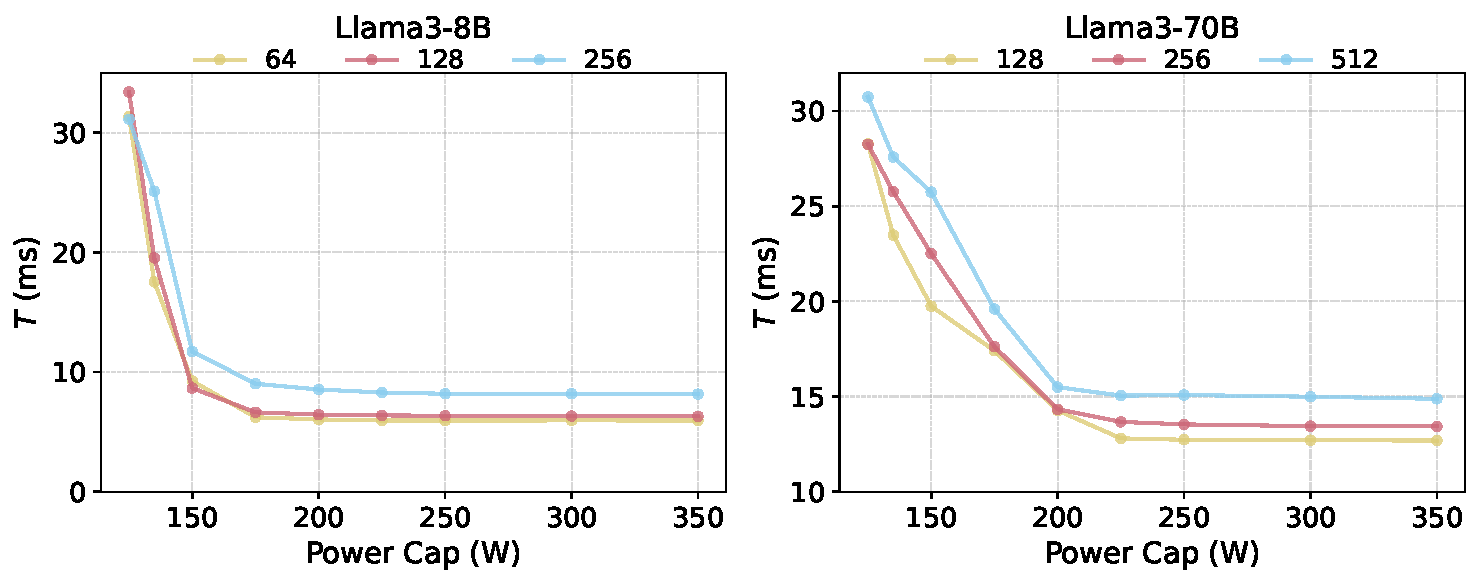
\includegraphics[width=1\linewidth]{figures/execution_time_sampling_new_new.pdf}
%     \caption{Variation of $T$ with different batch size across four Nvidia RTX 3090 GPUs and one NVidia A100 GPU, using Llama3-8B and Llama3-70B on the ShareGPT dataset.}
%     \label{profile_data}
% \end{figure}


We collect data on four NVIDIA RTX 3090 GPUs running Llama3-8B and eight NVIDIA A100 GPUs running Llama3-70B.
The ShareGPT dataset\cite{chiang2023vicuna} was utilized as the primary workload.
During the measurements, we set the frequency for the GPUs in all stages except the last one prior to launching the inference tasks. 
Key timestamps, such as the start and the end for each batch $B_{i,j}^{k}$ across all GPU stages were recorded.

Our analysis focuses specifically on the execution time of every iteration in the first three stages of a batch.
Since the first three stages have the same number of layers and are executed on the same GPU hardware, their execution times are assumed to be the same and stable as discussed in Section~\ref{sec:stableexecutiontime} . 
For simplicity, we denote the execution time of each stage as $T$. 
We subsequently analyzed the relationship between $T$ and $f$ under varying batch sizes.
We conducted multiple experiments with the batch size ranging from \hcwplaceholder{XX} to \hcwplaceholder{XXX}.
For each configuration, the GPU frequency was adjusted from \hcwplaceholder{XXX}Hz to \hcwplaceholder{XXX}Hz.
The detailed results are presented in Figure~\ref{profile_data}.

%实验环境，写好了
% \begin{figure}[t]
%     \centering
%     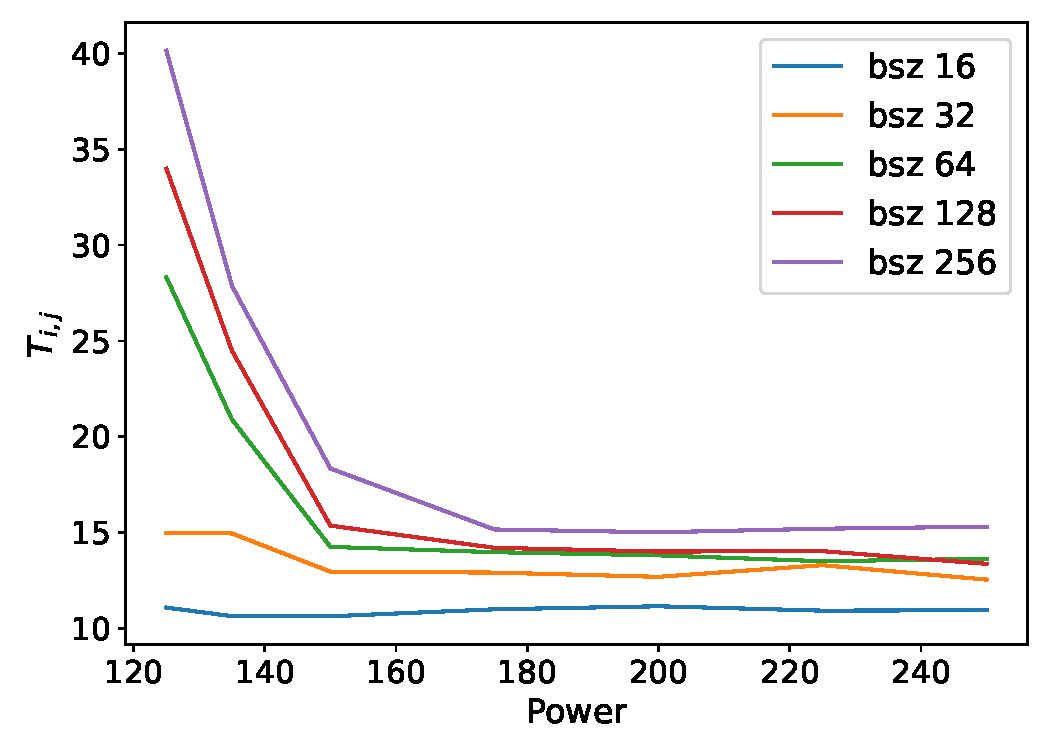
\includegraphics[width=0.8\linewidth]{figures/profile_power.pdf}
%     \caption{The impact of different powers on $T$ at multiple batch sizes}
%     \label{profile_power}
% \end{figure}


Based on the data collected, \thisproj{} was used to build an analytical model for the relationship between $T$ and $f$.
We name it as \textit{TFPrediction Model}.
The model can be formulated as follows: 
\begin{equation}
T=k_1*e^{-k_2f}+k_3
\label{model}
\end{equation} where $k_1$,$k_2$,$k_3$ are coefficients determined by profiling.

% 具体陈述背景ing

We also collect additional data for each batch size to validate the model's effectiveness and to assess its accuracy. By comparing the actual value at each different frequency setting with the value predicted by the \textit{TFPrediction Model}, we found that the \emph{Mean Absolute Percentage
Error (MAPE)} of the predictions is within \hcwplaceholder{XXX}\% on average, which we will further discuss in Section \ref{sec:evaluatecurvefitting}.
It is important to note that, although the batch size can influence the \textit{TFPrediction Model}, its values are discrete rather than continuous making them unsuitable for curve-fitting-based predictions. 
Consequently, the \thisproj{} excludes the batch size as a parameter in the \textit{TFPrediction Model}.



\subsection{Model-Guided Energy Efficiency Optimization}
\label{sec:guide}

Once the analytical model between $T$ and $f$ is established, we can use it to guide the frequency adjustments. 
Based on the analysis in Section~\ref{Principle Model}, the execution time of the last stage $T_{i,N}^{k}$, and the CPU scheduling time $T_S$ are also critical parameters in configuring the frequency.
%The data collected from the profiling and modeling is retained for this purpose. 
Since no frequency adjustment is applied to the GPU that handles the last stage of the inference, its execution time $T_{i,N}^{k}$ remains the same before and after the frequency adjustment.
Similarly, the scheduling time $T_S$, which depends on the time required for each token generation task, is also unaffected. 
This is because the GPU frequency management only slows down each stage to reduce bubbles, but will leave the critical path for the token generation unchanged. 
Thus, $T_S$ is considered constant before and after GPU frequency adjustments.
Based on this observation, all we need is to configure GPU frequency to align $T_{i,1}^{k}$ with $T_{i,N}^{k} - T_S$ and adjust the other stages $T_{i,2}^{k}$ through $T_{i,N-1}^{k}$ to match $T_{i,N}^{k}$.



\subsection{Universality of the Model}
\label{sec:modelportable}


Notably, as the critical parameters of the GPU frequency configuration that include $T$, $T_S$ and the model parameters from the \textit{TFPrediction Model} are collected from profiling, it is important to know how they are affected by the LLM inference execution environment.
It can determine the generalizability of our model, specifically whether it can effectively and efficiently enhance the inference engine with a minimal profiling overhead.

The execution time of an application is generally influenced by its input data and the software and hardware configurations \cite{fu2024serverlessllm,moon2024lpu}. 
For an LLM inference engine, they can be categorized as follows.
\textbf{Input data:} The requests submitted by users, such as the texts of the questions posted, may directly impact the execution time.
\textbf{Software configurations:} Key factors may include the batching strategy, the batch size and the model scale.
% , and other parameters \bygxl{list additional relevant factors here}.
% GPU memory
\textbf{Hardware configurations:} The type and the number of GPUs, which determine the number of pipeline stages, can significantly affect the performance.
Understanding the interplay of these factors is critical in understanding how the key parameters work in \thisproj{}.


Firstly, the input data directly determines the \textit{sequence length} of each request.
As discussed in Section~\ref{sec:stableexecutiontime}, the execution time is generally insensitive to sequence length.
Therefore, we neglect the impact of \textbf{input data} in \thisproj{}.


For the \textbf{Software configuration}, model scale and batch size influence the size of the matrices involved in computation, consequently impacting execution time, as analyzed in Section~\ref{sec:llmandtransformer}.
% Specifically, the model scale dictates the size of the parameter matrix, while the batch size controls the number of rows in the QKV matrix.
\bylyz{Specifically, the model scale determines the size of the parameter matrices, whereas the batch size dictates the size of the input matrices.}
Although these factors have a significant impact on $T$, they are typically determined before the deployment of LLMs and remain fixed throughout the inference process.
Consequently, $T$ requires only an one-time profiling for each combination of the model and the batch size.
In practice, the diversity of LLMs is limited by training cost, and the choice of batch size is constrained by GPU memory, further reducing profiling effort. 



\textbf{Hardware features} also play a critical role in determining the execution time and the energy efficiency of batches. 
% Consequently, re-profiling $T_{i,n}$ becomes necessary when the hardware platform changes.
Consequently, re-profiling $T$ is required when the hardware platform changes.
Similarly, the \textit{TFPrediction Model}, which is vital for predicting batch execution times, is also insensitive to input data. 
% Instead, it is primarily influenced by software configurations such as Model Scale, Batch Size (bsz), and hardware features. 
Instead, it is primarily influenced by software configurations such as model scale, batch size, and hardware features. 
Re-profiling is required whenever these parameters change. 
% However, as the shape of the curve is inherently determined by the characteristics of the GPU, our experiments demonstrated that only six measurements are needed to achieve adequate accuracy for the model.
However, as the shape of the curve is inherently determined by the characteristics of the GPU, our experiments show that only six measurements are needed to achieve adequate accuracy for the model.
% \bygxl{only XXXX measurements are needed to parameterize the model}.

For $T_S$, its execution time is determined by the CPU and the number of requests to be scheduled, which in turn are influenced by both the hardware and the batch size. 
As noted earlier, in an on-going inference, neither the batch size nor the hardware changes. 
Hence, once the operating environment is established, $T_S$ requires only an one-time profiling.


In summary, the batch-level behavior is insensitive to the input data and is primarily influenced by the software configuration and the hardware platform.  
As these parameters remain stable in an ongoing inference environment, a one-time profiling effort is sufficient to ensure the applicability of our model to subsequent inference runs. 


